\documentclass[aspectratio=169]{beamer}

\usetheme{default}
\usecolortheme{dove}

\setbeamertemplate{navigation symbols}{}
\setbeamertemplate{footline}{%
  \hfill{\large\insertframenumber\,/\,\inserttotalframenumber}\hspace{0.8em}\vspace{0.5em}%
}

\definecolor{popblue}{RGB}{52, 101, 164}
\definecolor{sampred}{RGB}{204, 0, 0}
\definecolor{paramgreen}{RGB}{0, 140, 70}
\definecolor{warnred}{RGB}{180, 40, 40}
\definecolor{orange1}{RGB}{220, 120, 0}
\definecolor{violet1}{RGB}{120, 50, 160}
\definecolor{lightbg}{RGB}{245, 245, 250}

\setbeamercolor{frametitle}{fg=popblue}
\setbeamercolor{title}{fg=popblue}

\usepackage{pgfplots}
\usepackage{tikz}
\usetikzlibrary{shapes, arrows.meta, positioning, calc, decorations.pathreplacing, patterns}
\pgfplotsset{compat=1.18}
\usepackage{amsmath, amssymb}
\usepackage{pifont}
\usepackage{colortbl}
\usepackage{fontenc}

\title{Lecture 13: Generalized Linear Models}
\subtitle{One Framework $\cdot$ Three Components $\cdot$ Many Models}
\date{}

\begin{document}

% ============================================================
\begin{frame}
\titlepage
\end{frame}

% ============================================================
\begin{frame}
\frametitle{Previously, on Lecture 12\ldots}

\begin{center}
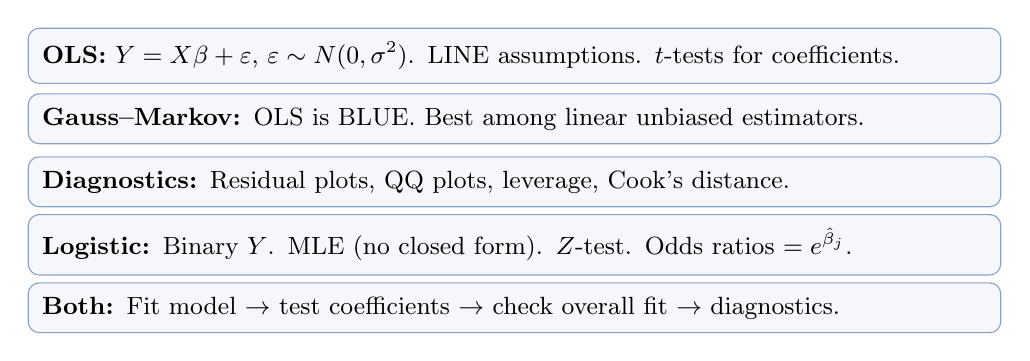
\begin{tikzpicture}[
  sbox/.style={draw=popblue!60, fill=popblue!5, rounded corners=4pt, text width=12cm, minimum height=0.5cm, align=left, inner sep=5pt, font=\small}
]
  \node[sbox] at (0, 2.0) {\textbf{OLS:} $Y = X\beta + \varepsilon$, $\varepsilon \sim N(0, \sigma^2)$. LINE assumptions. $t$-tests for coefficients.};
  \node[sbox] at (0, 1.2) {\textbf{Gauss--Markov:} OLS is BLUE. Best among linear unbiased estimators.};
  \node[sbox] at (0, 0.4) {\textbf{Diagnostics:} Residual plots, QQ plots, leverage, Cook's distance.};
  \node[sbox] at (0, -0.4) {\textbf{Logistic:} Binary $Y$. MLE (no closed form). $Z$-test. Odds ratios $= e^{\hat\beta_j}$.};
  \node[sbox] at (0, -1.2) {\textbf{Both:} Fit model $\to$ test coefficients $\to$ check overall fit $\to$ diagnostics.};
\end{tikzpicture}
\end{center}

\vspace{0.3cm}
\begin{center}
{\large\textbf{Today:}} OLS and logistic regression look different --- but they are\\
\textbf{the same machine} with different settings. That machine is the GLM.
\end{center}
\end{frame}

% ============================================================
% PART I: MOTIVATION
% ============================================================
\section{Why GLMs?}

\begin{frame}
\begin{center}
  \vspace{1.5cm}
  {\Huge\bfseries\textcolor{popblue}{Part I: Why Do We Need GLMs?}}

  \vspace{0.8cm}
  {\large Not all data is Normal. Not all relationships are linear.}
\end{center}
\end{frame}

\begin{frame}
\frametitle{Three Problems, Three Response Types}

\begin{center}
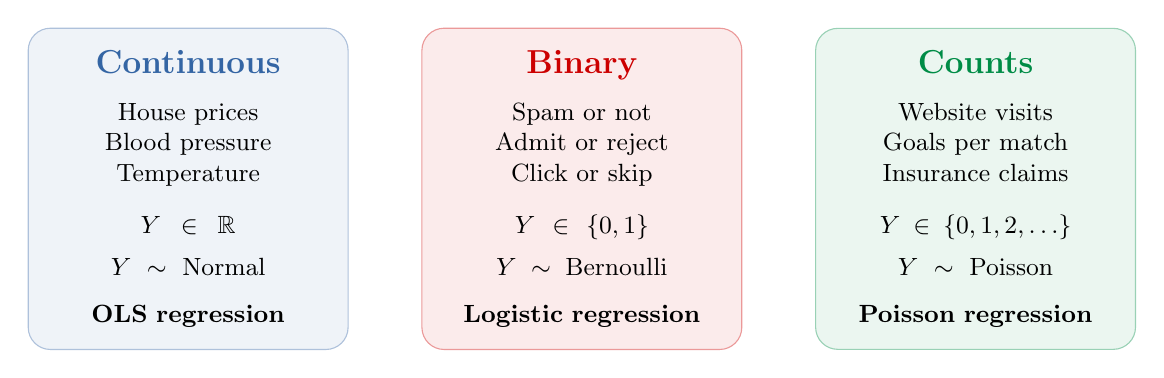
\begin{tikzpicture}[
  pbox/.style={draw, rounded corners=8pt, text width=3.5cm, align=center, inner sep=8pt, font=\small, minimum height=4cm}
]
  \node[pbox, fill=popblue!8, draw=popblue!40] at (-5, 0) {
    {\large\bfseries\textcolor{popblue}{Continuous}}\\[6pt]
    House prices\\
    Blood pressure\\
    Temperature\\[8pt]
    $Y \in \mathbb{R}$\\[4pt]
    $Y \sim \text{Normal}$\\[6pt]
    \textbf{OLS regression}
  };
  \node[pbox, fill=sampred!8, draw=sampred!40] at (0, 0) {
    {\large\bfseries\textcolor{sampred}{Binary}}\\[6pt]
    Spam or not\\
    Admit or reject\\
    Click or skip\\[8pt]
    $Y \in \{0, 1\}$\\[4pt]
    $Y \sim \text{Bernoulli}$\\[6pt]
    \textbf{Logistic regression}
  };
  \node[pbox, fill=paramgreen!8, draw=paramgreen!40] at (5, 0) {
    {\large\bfseries\textcolor{paramgreen}{Counts}}\\[6pt]
    Website visits\\
    Goals per match\\
    Insurance claims\\[8pt]
    $Y \in \{0, 1, 2, \ldots\}$\\[4pt]
    $Y \sim \text{Poisson}$\\[6pt]
    \textbf{Poisson regression}
  };
\end{tikzpicture}
\end{center}

\vspace{0.2cm}
\begin{center}
\fcolorbox{popblue}{popblue!5}{\parbox{10cm}{\centering\small
  All three are \textbf{special cases of one framework}: the Generalized Linear Model.\\
  Same estimation (MLE), same inference ($Z$-tests, CIs), same diagnostics.
}}
\end{center}
\end{frame}

\begin{frame}
\frametitle{Why Not Just Use OLS for Everything?}

\begin{center}
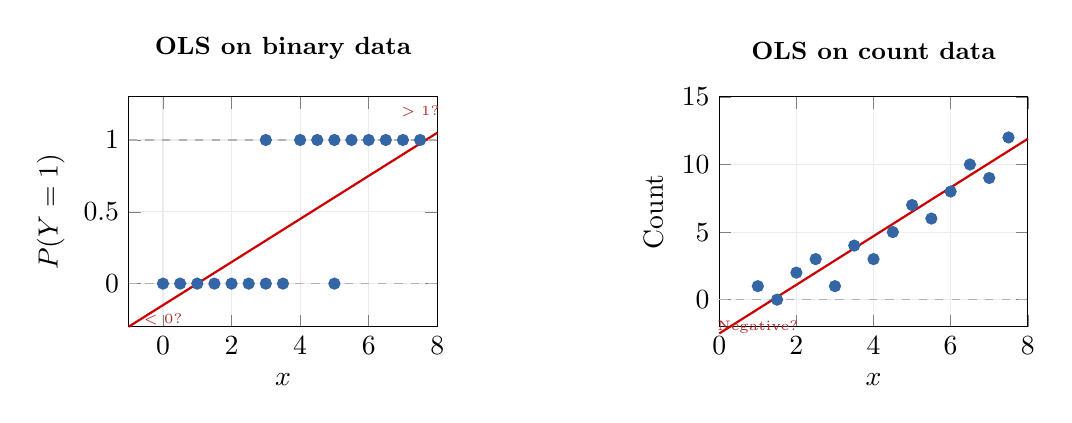
\begin{tikzpicture}
  % Binary data with OLS line
  \begin{axis}[
    width=5.5cm, height=4.5cm,
    xlabel={$x$}, ylabel={$P(Y=1)$},
    xmin=-1, xmax=8, ymin=-0.3, ymax=1.3,
    grid=major, grid style={gray!15},
    title={\small\textbf{OLS on binary data}},
    title style={at={(0.5,1.05)}},
    clip=false
  ]
    \addplot[only marks, mark=*, mark size=2pt, popblue] coordinates {
      (0,0) (0.5,0) (1,0) (1.5,0) (2,0) (2.5,0) (3,0) (3,1) (3.5,0) (4,1)
      (4.5,1) (5,1) (5,0) (5.5,1) (6,1) (6.5,1) (7,1) (7.5,1)
    };
    \addplot[sampred, thick, domain=-1:8] {-0.15 + 0.15*x};
    \draw[dashed, black!30] (axis cs:-1, 0) -- (axis cs:8, 0);
    \draw[dashed, black!30] (axis cs:-1, 1) -- (axis cs:8, 1);
    \node[font=\tiny, warnred] at (axis cs:7.5, 1.2) {$> 1$?};
    \node[font=\tiny, warnred] at (axis cs:0, -0.25) {$< 0$?};
  \end{axis}

  % Count data with OLS line
  \begin{scope}[shift={(7.5, 0)}]
  \begin{axis}[
    width=5.5cm, height=4.5cm,
    xlabel={$x$}, ylabel={Count},
    xmin=0, xmax=8, ymin=-2, ymax=15,
    grid=major, grid style={gray!15},
    title={\small\textbf{OLS on count data}},
    title style={at={(0.5,1.05)}},
    clip=false
  ]
    \addplot[only marks, mark=*, mark size=2pt, popblue] coordinates {
      (1,1) (1.5,0) (2,2) (2.5,3) (3,1) (3.5,4) (4,3) (4.5,5)
      (5,7) (5.5,6) (6,8) (6.5,10) (7,9) (7.5,12)
    };
    \addplot[sampred, thick, domain=0:8] {-2.5 + 1.8*x};
    \draw[dashed, black!30] (axis cs:0, 0) -- (axis cs:8, 0);
    \node[font=\tiny, warnred] at (axis cs:1, -2) {Negative?};
  \end{axis}
  \end{scope}
\end{tikzpicture}
\end{center}

\vspace{0.1cm}
\begin{center}
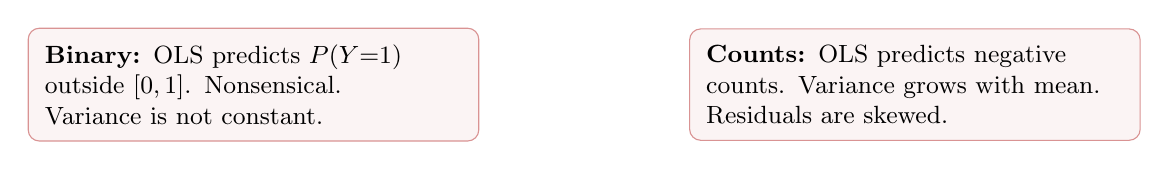
\begin{tikzpicture}[
  fbox/.style={draw=warnred!50, fill=warnred!5, rounded corners=4pt, text width=5.3cm, align=left, inner sep=6pt, font=\small}
]
  \node[fbox] at (-4.2, 0) {
    \textbf{Binary:} OLS predicts $P(Y{=}1)$\\
    outside $[0, 1]$. Nonsensical.\\
    Variance is not constant.
  };
  \node[fbox] at (4.2, 0) {
    \textbf{Counts:} OLS predicts negative\\
    counts. Variance grows with mean.\\
    Residuals are skewed.
  };
\end{tikzpicture}
\end{center}
\end{frame}

% ============================================================
% PART II: THE THREE COMPONENTS
% ============================================================
\section{The GLM Framework}

\begin{frame}
\begin{center}
  \vspace{1.5cm}
  {\Huge\bfseries\textcolor{popblue}{Part II: The Three Components}}

  \vspace{0.8cm}
  {\large Random + Systematic + Link = GLM}
\end{center}
\end{frame}

\begin{frame}
\frametitle{The Three Components of a GLM}

\begin{center}
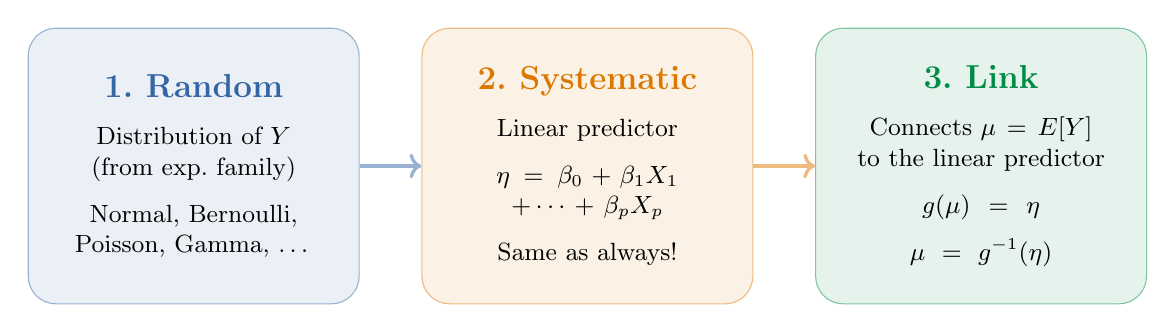
\begin{tikzpicture}[
  cbox/.style={draw, rounded corners=10pt, text width=3.5cm, align=center, inner sep=10pt, font=\small, minimum height=3.5cm}
]
  \node[cbox, fill=popblue!10, draw=popblue!50] (rand) at (-5, 0) {
    {\large\bfseries\textcolor{popblue}{1. Random}}\\[6pt]
    Distribution of $Y$\\
    (from exp.\ family)\\[6pt]
    Normal, Bernoulli,\\
    Poisson, Gamma, \ldots
  };
  \node[cbox, fill=orange1!10, draw=orange1!50] (sys) at (0, 0) {
    {\large\bfseries\textcolor{orange1}{2. Systematic}}\\[6pt]
    Linear predictor\\[6pt]
    $\eta = \beta_0 + \beta_1 X_1$\\
    $+ \cdots + \beta_p X_p$\\[6pt]
    Same as always!
  };
  \node[cbox, fill=paramgreen!10, draw=paramgreen!50] (link) at (5, 0) {
    {\large\bfseries\textcolor{paramgreen}{3. Link}}\\[6pt]
    Connects $\mu = E[Y]$\\
    to the linear predictor\\[6pt]
    $g(\mu) = \eta$\\[6pt]
    $\mu = g^{-1}(\eta)$
  };

  \draw[->, very thick, popblue!50] (rand) -- (sys);
  \draw[->, very thick, orange1!50] (sys) -- (link);
\end{tikzpicture}
\end{center}

\vspace{0.2cm}
\begin{center}
\fcolorbox{violet1}{violet1!5}{\parbox{10cm}{\centering\small
  \textbf{Key insight:} We don't model $Y$ directly as linear in $X$.\\
  Instead, we model some \textbf{transformation} $g(\mu)$ as linear in $X$.\\
  The link function $g$ ensures predictions make sense for the data type.
}}
\end{center}
\end{frame}

\begin{frame}
\frametitle{Exponential Family: The Common Thread}
\framesubtitle{Connects to L3 (exponential family) and L5 (MLE)}

\begin{center}
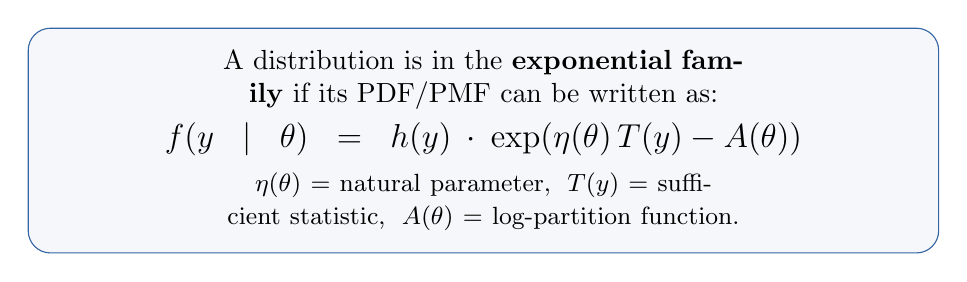
\begin{tikzpicture}
  \node[draw=popblue, fill=popblue!5, rounded corners=8pt, text width=11cm, align=center, inner sep=8pt] {
    A distribution is in the \textbf{exponential family} if its PDF/PMF can be written as:\\[4pt]
    {\large $f(y \mid \theta) = h(y) \cdot \exp\!\left(\eta(\theta)\, T(y) - A(\theta)\right)$}\\[4pt]
    \small $\eta(\theta)$ = natural parameter, \;$T(y)$ = sufficient statistic, \;$A(\theta)$ = log-partition function.
  };
\end{tikzpicture}
\end{center}

\vspace{0.1cm}
\begin{center}
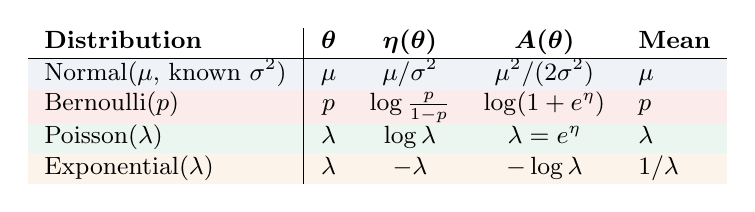
\begin{tikzpicture}
  \node[inner sep=0pt] {
    \small
    \begin{tabular}{l|cccl}
      \textbf{Distribution} & $\boldsymbol{\theta}$ & $\boldsymbol{\eta(\theta)}$ & $\boldsymbol{A(\theta)}$ & \textbf{Mean} \\
      \hline
      \rowcolor{popblue!8}
      Normal($\mu$, known $\sigma^2$) & $\mu$ & $\mu/\sigma^2$ & $\mu^2/(2\sigma^2)$ & $\mu$ \\
      \rowcolor{sampred!8}
      Bernoulli($p$) & $p$ & $\log\frac{p}{1-p}$ & $\log(1+e^\eta)$ & $p$ \\
      \rowcolor{paramgreen!8}
      Poisson($\lambda$) & $\lambda$ & $\log\lambda$ & $\lambda = e^\eta$ & $\lambda$ \\
      \rowcolor{orange1!8}
      Exponential($\lambda$) & $\lambda$ & $-\lambda$ & $-\log\lambda$ & $1/\lambda$ \\
    \end{tabular}
  };
\end{tikzpicture}
\end{center}

\vspace{0.1cm}
\begin{center}
\small The \textbf{canonical link} sets $g(\mu) = \eta(\theta)$: the natural parameter \textit{is} the linear predictor.
\end{center}
\end{frame}

\begin{frame}
\frametitle{Link Functions: The Key Examples}

\begin{center}
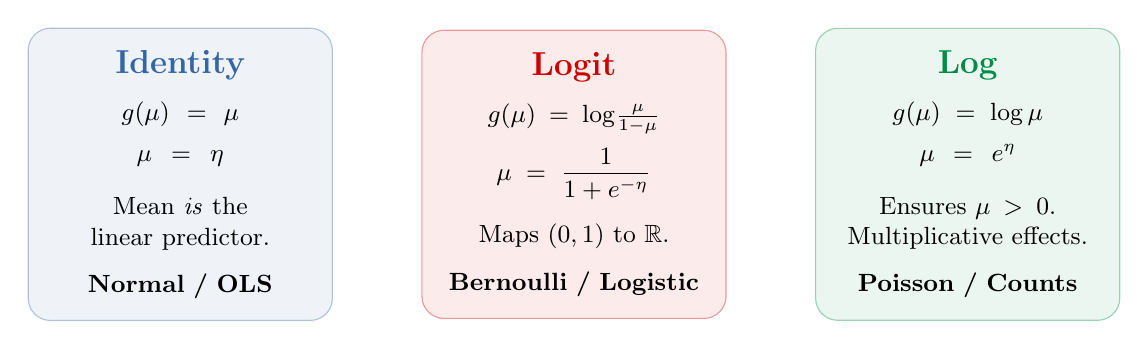
\begin{tikzpicture}[
  lbox/.style={draw, rounded corners=8pt, text width=3.3cm, align=center, inner sep=8pt, font=\small, minimum height=3.5cm}
]
  \node[lbox, fill=popblue!8, draw=popblue!40] at (-5, 0) {
    {\large\bfseries\textcolor{popblue}{Identity}}\\[6pt]
    $g(\mu) = \mu$\\[4pt]
    $\mu = \eta$\\[8pt]
    Mean \textit{is} the\\
    linear predictor.\\[6pt]
    \textbf{Normal / OLS}
  };
  \node[lbox, fill=sampred!8, draw=sampred!40] at (0, 0) {
    {\large\bfseries\textcolor{sampred}{Logit}}\\[6pt]
    $g(\mu) = \log\!\frac{\mu}{1-\mu}$\\[4pt]
    $\mu = \dfrac{1}{1+e^{-\eta}}$\\[8pt]
    Maps $(0,1)$ to $\mathbb{R}$.\\[6pt]
    \textbf{Bernoulli / Logistic}
  };
  \node[lbox, fill=paramgreen!8, draw=paramgreen!40] at (5, 0) {
    {\large\bfseries\textcolor{paramgreen}{Log}}\\[6pt]
    $g(\mu) = \log\mu$\\[4pt]
    $\mu = e^{\eta}$\\[8pt]
    Ensures $\mu > 0$.\\
    Multiplicative effects.\\[6pt]
    \textbf{Poisson / Counts}
  };
\end{tikzpicture}
\end{center}

\vspace{0.2cm}
\begin{center}
\fcolorbox{orange1}{orange1!5}{\parbox{10cm}{\centering\small
  These are the \textbf{canonical links} --- the ``natural'' choice for each distribution.\\
  Other links exist (probit for binary, inverse for Gamma), but canonical is the default.
}}
\end{center}
\end{frame}

% ============================================================
% PART III: OLS AS A GLM
% ============================================================
\section{OLS as a GLM}

\begin{frame}
\begin{center}
  \vspace{1.5cm}
  {\Huge\bfseries\textcolor{popblue}{Part III: OLS Is a GLM}}

  \vspace{0.8cm}
  {\large Everything you already know, rewritten in GLM language}
\end{center}
\end{frame}

\begin{frame}
\frametitle{Linear Regression = GLM(Normal, Identity)}

\begin{center}
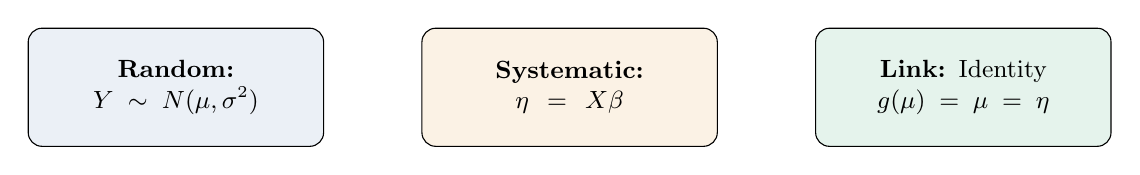
\begin{tikzpicture}[
  cbox/.style={draw, rounded corners=5pt, text width=3.4cm, align=center, inner sep=5pt, font=\small, minimum height=1.5cm}
]
  \node[cbox, fill=popblue!10] at (-5, 0) {
    \textbf{Random:}\\
    $Y \sim N(\mu, \sigma^2)$
  };
  \node[cbox, fill=orange1!10] at (0, 0) {
    \textbf{Systematic:}\\
    $\eta = X\beta$
  };
  \node[cbox, fill=paramgreen!10] at (5, 0) {
    \textbf{Link:} Identity\\
    $g(\mu) = \mu = \eta$
  };
\end{tikzpicture}
\end{center}

\vspace{0.1cm}
\begin{center}
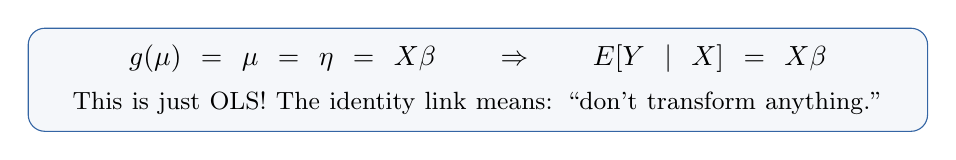
\begin{tikzpicture}
  \node[draw=popblue, fill=popblue!5, rounded corners=6pt, text width=11cm, align=center, inner sep=6pt] {
    $g(\mu) = \mu = \eta = X\beta$ \qquad $\Rightarrow$ \qquad $E[Y \mid X] = X\beta$\\[4pt]
    {\small This is just OLS! The identity link means: ``don't transform anything.''}
  };
\end{tikzpicture}
\end{center}

\vspace{0.1cm}
\begin{center}
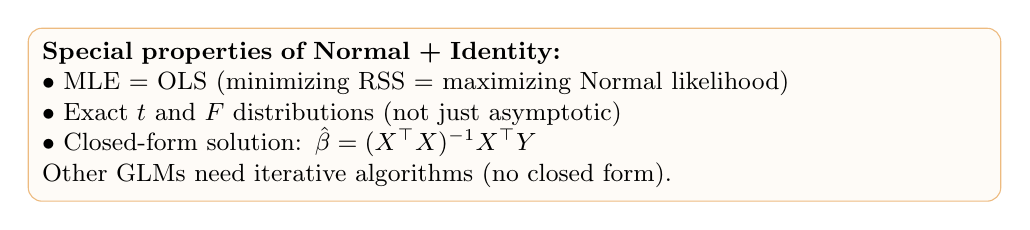
\begin{tikzpicture}
  \node[draw=orange1!50, fill=orange1!3, rounded corners=5pt, text width=12cm, align=left, inner sep=5pt, font=\small] {
    \textbf{Special properties of Normal + Identity:}\\
    $\bullet$ MLE $=$ OLS (minimizing RSS $=$ maximizing Normal likelihood)\\
    $\bullet$ Exact $t$ and $F$ distributions (not just asymptotic)\\
    $\bullet$ Closed-form solution: $\hat\beta = (X^\top X)^{-1} X^\top Y$\\
    Other GLMs need iterative algorithms (no closed form).
  };
\end{tikzpicture}
\end{center}
\end{frame}

% ============================================================
% PART IV: LOGISTIC AS A GLM
% ============================================================
\section{Logistic as a GLM}

\begin{frame}
\begin{center}
  \vspace{1.5cm}
  {\Huge\bfseries\textcolor{popblue}{Part IV: Logistic Is a GLM}}

  \vspace{0.8cm}
  {\large Same framework, different distribution and link}
\end{center}
\end{frame}

\begin{frame}
\frametitle{Logistic Regression = GLM(Bernoulli, Logit)}

\begin{center}
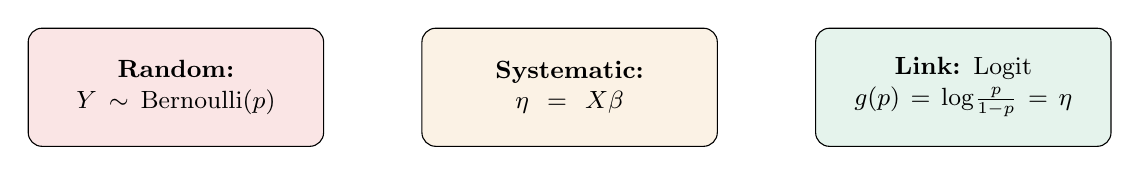
\begin{tikzpicture}[
  cbox/.style={draw, rounded corners=5pt, text width=3.4cm, align=center, inner sep=5pt, font=\small, minimum height=1.5cm}
]
  \node[cbox, fill=sampred!10] at (-5, 0) {
    \textbf{Random:}\\
    $Y \sim \text{Bernoulli}(p)$
  };
  \node[cbox, fill=orange1!10] at (0, 0) {
    \textbf{Systematic:}\\
    $\eta = X\beta$
  };
  \node[cbox, fill=paramgreen!10] at (5, 0) {
    \textbf{Link:} Logit\\
    $g(p) = \log\!\frac{p}{1-p} = \eta$
  };
\end{tikzpicture}
\end{center}

\vspace{0.1cm}
\begin{center}
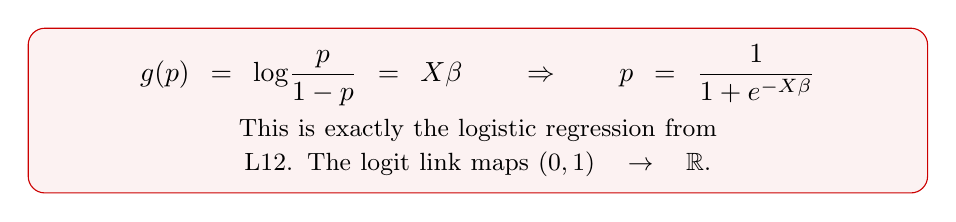
\begin{tikzpicture}
  \node[draw=sampred, fill=sampred!5, rounded corners=6pt, text width=11cm, align=center, inner sep=6pt] {
    $g(p) = \log\!\dfrac{p}{1-p} = X\beta$ \qquad $\Rightarrow$ \qquad $p = \dfrac{1}{1 + e^{-X\beta}}$\\[4pt]
    {\small This is exactly the logistic regression from L12. The logit link maps $(0,1) \to \mathbb{R}$.}
  };
\end{tikzpicture}
\end{center}

\vspace{0.1cm}
\begin{center}
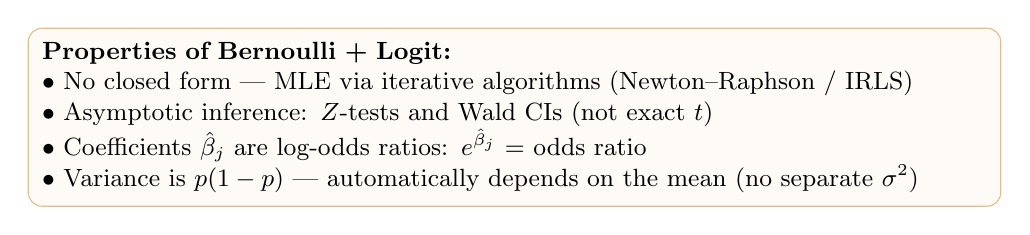
\begin{tikzpicture}
  \node[draw=orange1!50, fill=orange1!3, rounded corners=5pt, text width=12cm, align=left, inner sep=5pt, font=\small] {
    \textbf{Properties of Bernoulli + Logit:}\\
    $\bullet$ No closed form --- MLE via iterative algorithms (Newton--Raphson / IRLS)\\
    $\bullet$ Asymptotic inference: $Z$-tests and Wald CIs (not exact $t$)\\
    $\bullet$ Coefficients $\hat\beta_j$ are log-odds ratios: $e^{\hat\beta_j}$ = odds ratio\\
    $\bullet$ Variance is $p(1-p)$ --- automatically depends on the mean (no separate $\sigma^2$)
  };
\end{tikzpicture}
\end{center}
\end{frame}

% ============================================================
% PART V: POISSON REGRESSION
% ============================================================
\section{Poisson Regression}

\begin{frame}
\begin{center}
  \vspace{1.5cm}
  {\Huge\bfseries\textcolor{popblue}{Part V: Poisson Regression}}

  \vspace{0.8cm}
  {\large The new member of the GLM family: modeling counts}
\end{center}
\end{frame}

\begin{frame}
\frametitle{Poisson Regression = GLM(Poisson, Log)}

\begin{center}
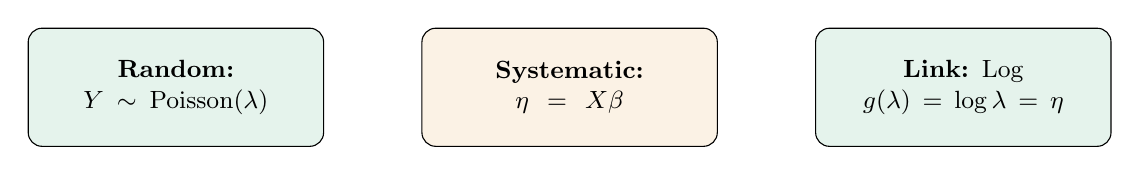
\begin{tikzpicture}[
  cbox/.style={draw, rounded corners=5pt, text width=3.4cm, align=center, inner sep=5pt, font=\small, minimum height=1.5cm}
]
  \node[cbox, fill=paramgreen!10] at (-5, 0) {
    \textbf{Random:}\\
    $Y \sim \text{Poisson}(\lambda)$
  };
  \node[cbox, fill=orange1!10] at (0, 0) {
    \textbf{Systematic:}\\
    $\eta = X\beta$
  };
  \node[cbox, fill=paramgreen!10] at (5, 0) {
    \textbf{Link:} Log\\
    $g(\lambda) = \log\lambda = \eta$
  };
\end{tikzpicture}
\end{center}

\vspace{0.1cm}
\begin{center}
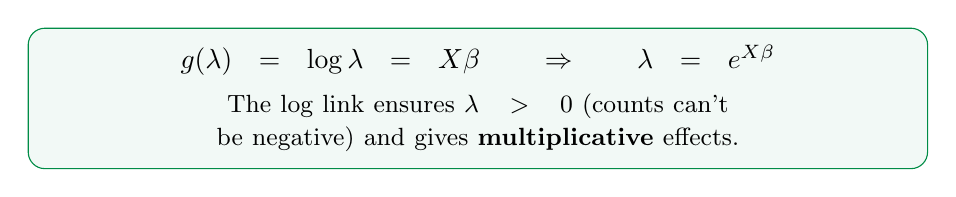
\begin{tikzpicture}
  \node[draw=paramgreen, fill=paramgreen!5, rounded corners=6pt, text width=11cm, align=center, inner sep=6pt] {
    $g(\lambda) = \log\lambda = X\beta$ \qquad $\Rightarrow$ \qquad $\lambda = e^{X\beta}$\\[4pt]
    {\small The log link ensures $\lambda > 0$ (counts can't be negative) and gives \textbf{multiplicative} effects.}
  };
\end{tikzpicture}
\end{center}

\vspace{0.1cm}
\begin{center}
\fcolorbox{orange1}{orange1!5}{\parbox{10cm}{\centering\small
  \textbf{Multiplicative interpretation:} A 1-unit increase in $X_j$ \textit{multiplies} the expected count by $e^{\beta_j}$.\\
  $e^{\beta_j} = 1.2$ means 20\% more events. $e^{\beta_j} = 0.8$ means 20\% fewer.\\
  This is the count analogue of the odds ratio in logistic regression.
}}
\end{center}
\end{frame}

\begin{frame}
\frametitle{Example: Bike Rentals}
\framesubtitle{Predicting daily bike rentals from temperature and weekday}

\small
$n = 365$ days. Model: $\log(\lambda_i) = \beta_0 + \beta_1 \cdot \text{Temp}_i + \beta_2 \cdot \text{Weekend}_i$.

\vspace{0.1cm}
\begin{center}
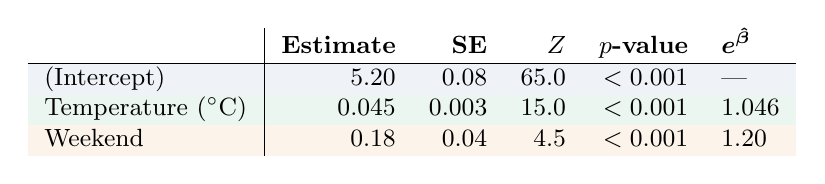
\begin{tikzpicture}
  \node[inner sep=0pt] {
    \small
    \begin{tabular}{l|rrrrl}
      & \textbf{Estimate} & \textbf{SE} & \textbf{$Z$} & \textbf{$p$-value} & $\boldsymbol{e^{\hat\beta}}$ \\
      \hline
      \rowcolor{popblue!8}
      (Intercept) & 5.20 & 0.08 & 65.0 & $< 0.001$ & --- \\
      \rowcolor{paramgreen!8}
      Temperature ($^\circ$C) & 0.045 & 0.003 & 15.0 & $< 0.001$ & 1.046 \\
      \rowcolor{orange1!8}
      Weekend & 0.18 & 0.04 & 4.5 & $< 0.001$ & 1.20 \\
    \end{tabular}
  };
\end{tikzpicture}
\end{center}

\vspace{0.15cm}
\begin{center}
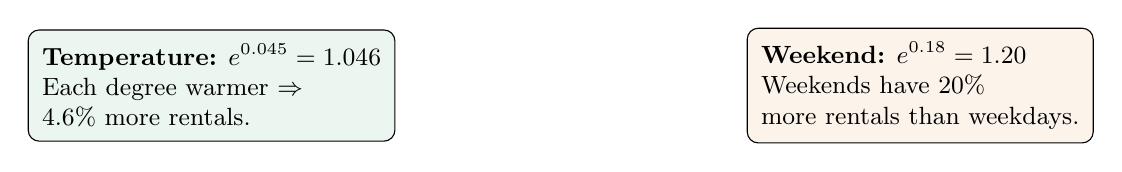
\begin{tikzpicture}[
  ibox/.style={draw, rounded corners=4pt, inner sep=5pt, font=\small, align=left}
]
  \node[ibox, fill=paramgreen!8] at (-4.5, 0) {
    \textbf{Temperature:} $e^{0.045} = 1.046$\\
    Each degree warmer $\Rightarrow$\\
    4.6\% more rentals.
  };
  \node[ibox, fill=orange1!8] at (4.5, 0) {
    \textbf{Weekend:} $e^{0.18} = 1.20$\\
    Weekends have 20\%\\
    more rentals than weekdays.
  };
\end{tikzpicture}
\end{center}

\vspace{0.1cm}
\small
At 20$^\circ$C on a weekday: $\hat\lambda = e^{5.20 + 0.045 \times 20 + 0.18 \times 0} = e^{6.10} \approx 446$ rentals.
\end{frame}

\begin{frame}
\frametitle{Poisson: Predicted vs Observed}

\begin{center}
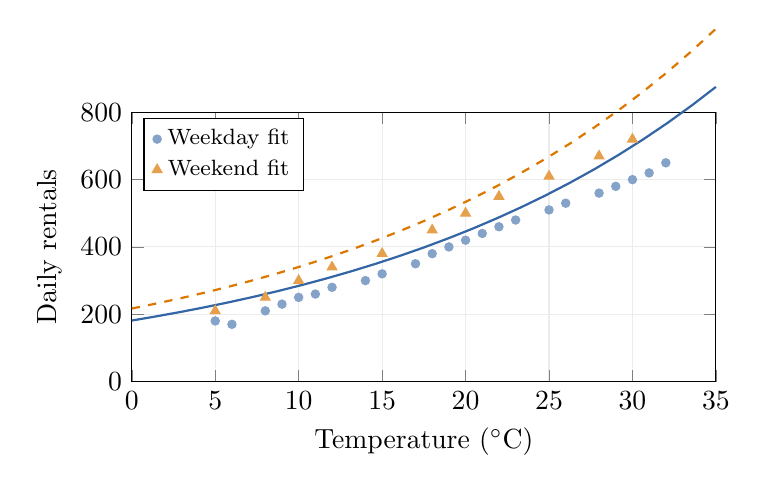
\begin{tikzpicture}
  \begin{axis}[
    width=9cm, height=5cm,
    xlabel={Temperature ($^\circ$C)},
    ylabel={Daily rentals},
    xmin=0, xmax=35, ymin=0, ymax=800,
    grid=major, grid style={gray!15},
    legend style={at={(0.02,0.98)}, anchor=north west, font=\footnotesize},
    clip=false
  ]
    % Weekday points
    \addplot[only marks, mark=*, mark size=1.5pt, popblue!60] coordinates {
      (5,180) (8,210) (10,250) (12,280) (15,320) (18,380) (20,420)
      (22,460) (25,510) (28,560) (30,600) (32,650)
      (6,170) (9,230) (11,260) (14,300) (17,350) (19,400) (21,440)
      (23,480) (26,530) (29,580) (31,620)
    };
    % Weekend points
    \addplot[only marks, mark=triangle*, mark size=2pt, orange1!70] coordinates {
      (5,210) (8,250) (10,300) (12,340) (15,380) (18,450) (20,500)
      (22,550) (25,610) (28,670) (30,720)
    };
    % Fitted curves
    \addplot[popblue, thick, domain=0:35] {exp(5.20 + 0.045*x)};
    \addlegendentry{Weekday fit}
    \addplot[orange1, thick, dashed, domain=0:35] {exp(5.20 + 0.045*x + 0.18)};
    \addlegendentry{Weekend fit}
  \end{axis}
\end{tikzpicture}
\end{center}

\vspace{0.1cm}
\begin{center}
\small The exponential curves naturally capture the \textbf{accelerating} relationship: more temperature = proportionally more rentals. OLS would predict a straight line.
\end{center}
\end{frame}

\begin{frame}
\frametitle{Overdispersion: When Poisson Isn't Enough}

\small
Poisson assumes $\text{Var}(Y) = \mu$. Real count data often has $\text{Var}(Y) > \mu$ (\textbf{overdispersion}).

\vspace{0.15cm}
\begin{center}
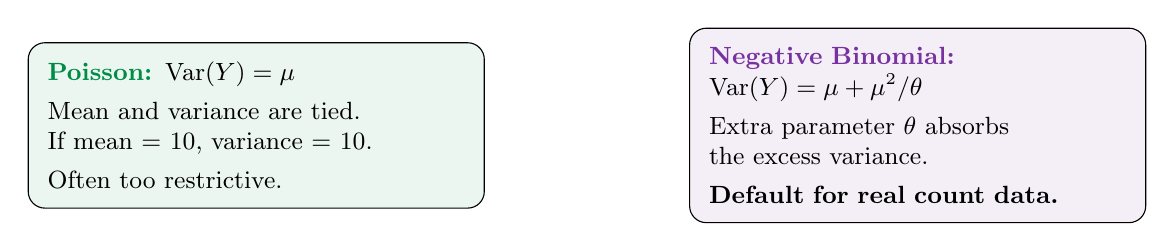
\begin{tikzpicture}[
  cbox/.style={draw, rounded corners=6pt, text width=5.3cm, align=left, inner sep=7pt, font=\small}
]
  \node[cbox, fill=paramgreen!8] at (-4.2, 0) {
    \textbf{\textcolor{paramgreen}{Poisson:}} $\text{Var}(Y) = \mu$\\[3pt]
    Mean and variance are tied.\\
    If mean = 10, variance = 10.\\[3pt]
    Often too restrictive.
  };
  \node[cbox, fill=violet1!8] at (4.2, 0) {
    \textbf{\textcolor{violet1}{Negative Binomial:}}\\
    $\text{Var}(Y) = \mu + \mu^2/\theta$\\[3pt]
    Extra parameter $\theta$ absorbs\\
    the excess variance.\\[3pt]
    \textbf{Default for real count data.}
  };
\end{tikzpicture}
\end{center}

\vspace{0.15cm}
\begin{center}
\fcolorbox{orange1}{orange1!5}{\parbox{10cm}{\centering\footnotesize
  \textbf{Diagnostic:} Fit Poisson, check residual deviance / df. If $\gg 1$: overdispersion.\\
  \textbf{Fix:} Use Negative Binomial (\texttt{statsmodels.GLM(family=NegativeBinomial())}) or\\
  Quasi-Poisson (same $\hat\beta$, inflated SEs).
}}
\end{center}
\end{frame}

% ============================================================
% PART VI: ESTIMATION & INFERENCE
% ============================================================
\section{Estimation \& Inference}

\begin{frame}
\begin{center}
  \vspace{1.5cm}
  {\Huge\bfseries\textcolor{popblue}{Part VI: How GLMs Are Fit}}

  \vspace{0.8cm}
  {\large MLE, IRLS, deviance, and the same inference workflow}
\end{center}
\end{frame}

\begin{frame}
\frametitle{MLE for GLMs: IRLS Algorithm}

\begin{center}
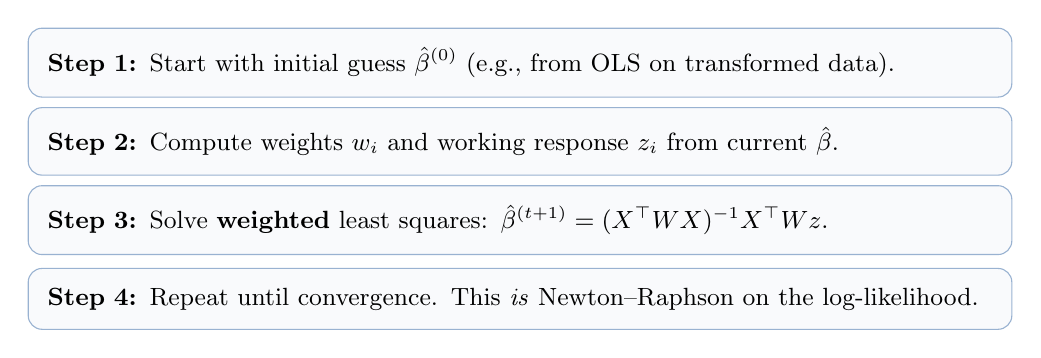
\begin{tikzpicture}[
  sbox/.style={draw=popblue!50, fill=popblue!3, rounded corners=5pt, text width=12cm, align=left, inner sep=7pt, font=\small}
]
  \node[sbox] at (0, 2.4) {
    \textbf{Step 1:} Start with initial guess $\hat\beta^{(0)}$ (e.g., from OLS on transformed data).
  };
  \node[sbox] at (0, 1.4) {
    \textbf{Step 2:} Compute weights $w_i$ and working response $z_i$ from current $\hat\beta$.
  };
  \node[sbox] at (0, 0.4) {
    \textbf{Step 3:} Solve \textbf{weighted} least squares: $\hat\beta^{(t+1)} = (X^\top W X)^{-1} X^\top W z$.
  };
  \node[sbox] at (0, -0.6) {
    \textbf{Step 4:} Repeat until convergence. This \textit{is} Newton--Raphson on the log-likelihood.
  };
\end{tikzpicture}
\end{center}

\vspace{0.1cm}
\begin{center}
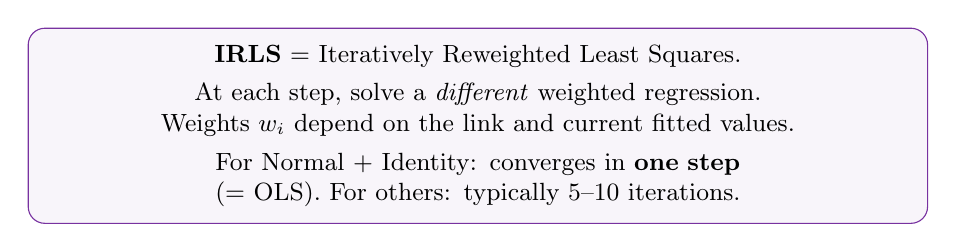
\begin{tikzpicture}
  \node[draw=violet1, fill=violet1!5, rounded corners=6pt, text width=11cm, align=center, inner sep=6pt, font=\small] {
    \textbf{IRLS} = Iteratively Reweighted Least Squares.\\[3pt]
    At each step, solve a \textit{different} weighted regression.
    Weights $w_i$ depend on the link and current fitted values.\\[3pt]
    For Normal + Identity: converges in \textbf{one step} (= OLS). For others: typically 5--10 iterations.
  };
\end{tikzpicture}
\end{center}
\end{frame}

\begin{frame}
\frametitle{Inference: Same Workflow, Different Details}

\begin{center}
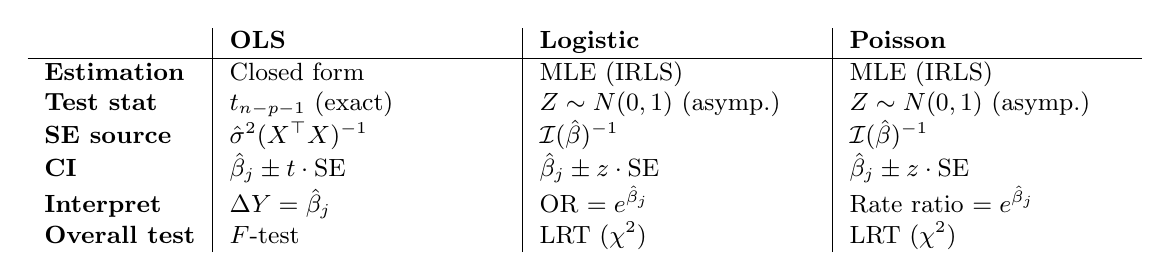
\begin{tikzpicture}
  \node[inner sep=0pt] {
    \small
    \begin{tabular}{l|p{3.5cm}|p{3.5cm}|p{3.5cm}}
      & \textbf{OLS} & \textbf{Logistic} & \textbf{Poisson} \\
      \hline
      \textbf{Estimation} & Closed form & MLE (IRLS) & MLE (IRLS) \\
      \textbf{Test stat} & $t_{n-p-1}$ (exact) & $Z \sim N(0,1)$ (asymp.) & $Z \sim N(0,1)$ (asymp.) \\
      \textbf{SE source} & $\hat\sigma^2(X^\top X)^{-1}$ & $\mathcal{I}(\hat\beta)^{-1}$ & $\mathcal{I}(\hat\beta)^{-1}$ \\
      \textbf{CI} & $\hat\beta_j \pm t \cdot \text{SE}$ & $\hat\beta_j \pm z \cdot \text{SE}$ & $\hat\beta_j \pm z \cdot \text{SE}$ \\
      \textbf{Interpret} & $\Delta Y = \hat\beta_j$ & OR $= e^{\hat\beta_j}$ & Rate ratio $= e^{\hat\beta_j}$ \\
      \textbf{Overall test} & $F$-test & LRT ($\chi^2$) & LRT ($\chi^2$) \\
    \end{tabular}
  };
\end{tikzpicture}
\end{center}

\vspace{0.2cm}
\begin{center}
\fcolorbox{popblue}{popblue!5}{\parbox{10cm}{\centering\small
  \textbf{The pattern is always the same:}\\
  Fit model $\to$ get $\hat\beta_j$ and SE $\to$ test $H_0\!: \beta_j = 0$ $\to$ CI $\to$ interpret $\to$ diagnostics.\\
  Only the distribution, link, and test statistic change.
}}
\end{center}
\end{frame}

\begin{frame}
\frametitle{Deviance: The GLM Analogue of RSS}

\begin{center}
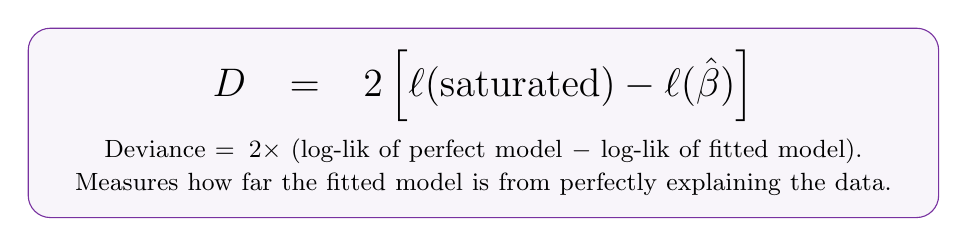
\begin{tikzpicture}
  \node[draw=violet1, fill=violet1!5, rounded corners=8pt, text width=11cm, align=center, inner sep=8pt] {
    {\Large $D = 2\left[\ell(\text{saturated}) - \ell(\hat\beta)\right]$}\\[5pt]
    \small Deviance $= 2 \times$ (log-lik of perfect model $-$ log-lik of fitted model).\\
    Measures how far the fitted model is from perfectly explaining the data.
  };
\end{tikzpicture}
\end{center}

\vspace{0.1cm}
\begin{center}
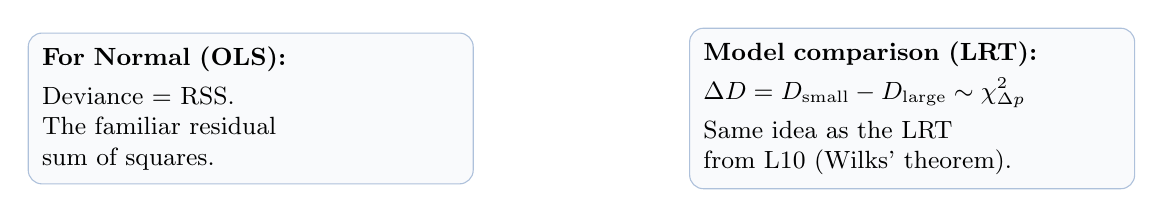
\begin{tikzpicture}[
  dbox/.style={draw=popblue!40, fill=popblue!3, rounded corners=5pt, text width=5.3cm, align=left, inner sep=5pt, font=\small}
]
  \node[dbox] at (-4.2, 0) {
    \textbf{For Normal (OLS):}\\[3pt]
    Deviance $=$ RSS.\\
    The familiar residual\\
    sum of squares.
  };
  \node[dbox] at (4.2, 0) {
    \textbf{Model comparison (LRT):}\\[3pt]
    $\Delta D = D_\text{small} - D_\text{large} \sim \chi^2_{\Delta p}$\\[3pt]
    Same idea as the LRT\\
    from L10 (Wilks' theorem).
  };
\end{tikzpicture}
\end{center}

\vspace{0.1cm}
\begin{center}
\small \textbf{AIC} $= D + 2p$ (penalize complexity). Lower AIC = better model. Replaces $R^2_\text{adj}$ for GLMs.
\end{center}
\end{frame}

% ============================================================
% PART VII: THE BIG PICTURE
% ============================================================
\section{The Big Picture}

\begin{frame}
\frametitle{The GLM Family Tree}

\begin{center}
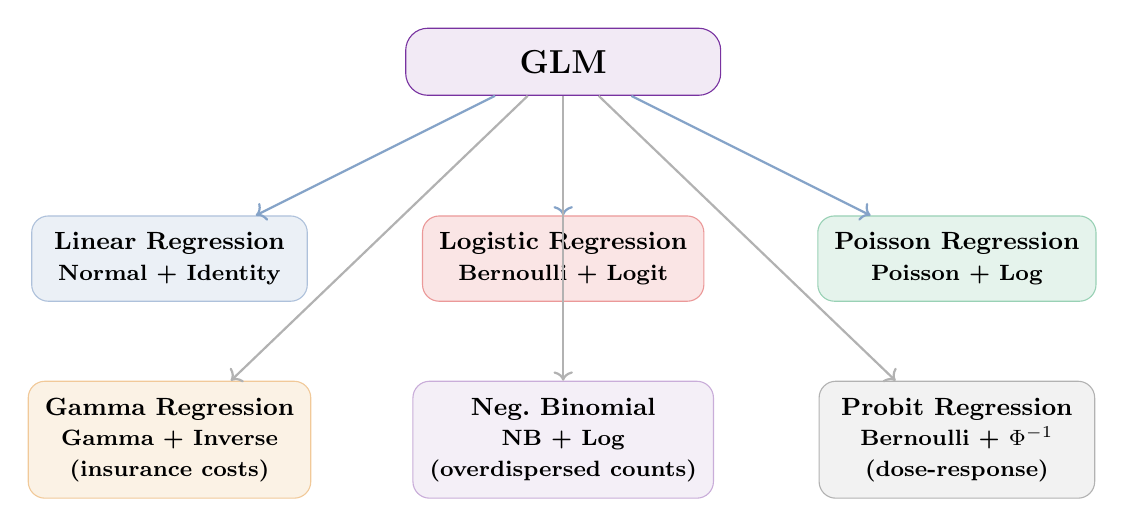
\begin{tikzpicture}[
  root/.style={draw=violet1, fill=violet1!10, rounded corners=8pt, inner sep=8pt, font=\large\bfseries, minimum width=4cm, align=center},
  child/.style={draw, rounded corners=6pt, inner sep=6pt, font=\small\bfseries, minimum width=3.5cm, align=center},
  arr/.style={->, thick, draw=popblue!60}
]
  \node[root] (glm) at (0, 3) {GLM};

  \node[child, fill=popblue!10, draw=popblue!40] (ols) at (-5, 0.5) {Linear Regression\\{\footnotesize Normal + Identity}};
  \node[child, fill=sampred!10, draw=sampred!40] (logit) at (0, 0.5) {Logistic Regression\\{\footnotesize Bernoulli + Logit}};
  \node[child, fill=paramgreen!10, draw=paramgreen!40] (pois) at (5, 0.5) {Poisson Regression\\{\footnotesize Poisson + Log}};

  \draw[arr] (glm) -- (ols);
  \draw[arr] (glm) -- (logit);
  \draw[arr] (glm) -- (pois);

  % Extensions
  \node[child, fill=orange1!10, draw=orange1!40] (gamma) at (-5, -1.8) {Gamma Regression\\{\footnotesize Gamma + Inverse}\\{\footnotesize (insurance costs)}};
  \node[child, fill=violet1!8, draw=violet1!40] (nb) at (0, -1.8) {Neg.\ Binomial\\{\footnotesize NB + Log}\\{\footnotesize (overdispersed counts)}};
  \node[child, fill=black!5, draw=black!30] (probit) at (5, -1.8) {Probit Regression\\{\footnotesize Bernoulli + $\Phi^{-1}$}\\{\footnotesize (dose-response)}};

  \draw[arr, draw=black!30] (glm) -- (gamma);
  \draw[arr, draw=black!30] (glm) -- (nb);
  \draw[arr, draw=black!30] (glm) -- (probit);
\end{tikzpicture}
\end{center}

\vspace{0.1cm}
\begin{center}
\small All share the same three-component structure. All use MLE. All have the same inference workflow.
\end{center}
\end{frame}

\begin{frame}
\frametitle{Choosing the Right GLM}

\begin{center}
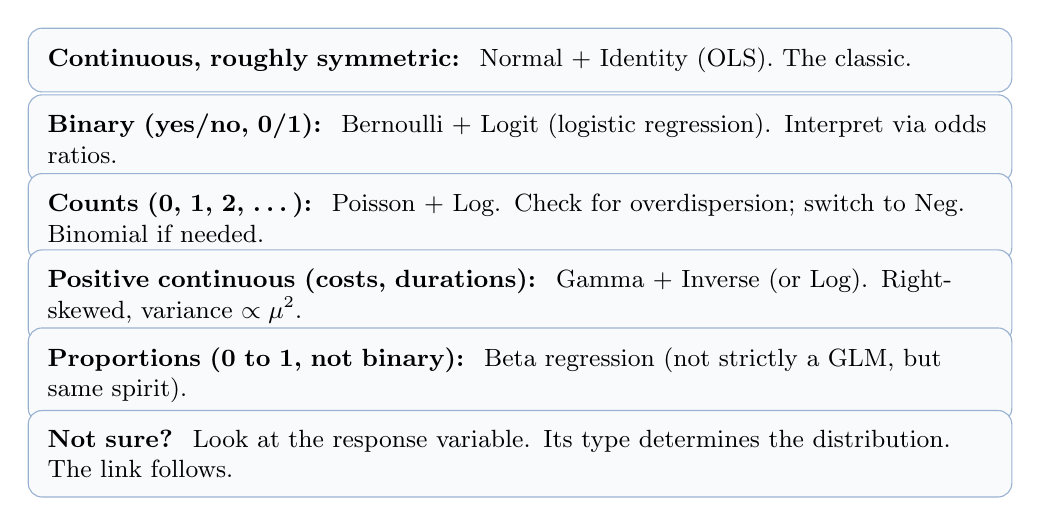
\begin{tikzpicture}[
  tbox/.style={draw=popblue!50, fill=popblue!3, rounded corners=5pt, text width=12cm, align=left, inner sep=7pt, font=\small}
]
  \node[tbox] at (0, 2.8) {
    \textbf{Continuous, roughly symmetric:}\;
    Normal + Identity (OLS). The classic.
  };
  \node[tbox] at (0, 1.8) {
    \textbf{Binary (yes/no, 0/1):}\;
    Bernoulli + Logit (logistic regression). Interpret via odds ratios.
  };
  \node[tbox] at (0, 0.8) {
    \textbf{Counts (0, 1, 2, \ldots):}\;
    Poisson + Log. Check for overdispersion; switch to Neg.\ Binomial if needed.
  };
  \node[tbox] at (0, -0.2) {
    \textbf{Positive continuous (costs, durations):}\;
    Gamma + Inverse (or Log). Right-skewed, variance $\propto \mu^2$.
  };
  \node[tbox] at (0, -1.2) {
    \textbf{Proportions (0 to 1, not binary):}\;
    Beta regression (not strictly a GLM, but same spirit).
  };
  \node[tbox] at (0, -2.2) {
    \textbf{Not sure?}\;
    Look at the response variable. Its type determines the distribution. The link follows.
  };
\end{tikzpicture}
\end{center}
\end{frame}

% ============================================================
\section{Summary}

\begin{frame}
\frametitle{Summary: Generalized Linear Models}
\begin{center}
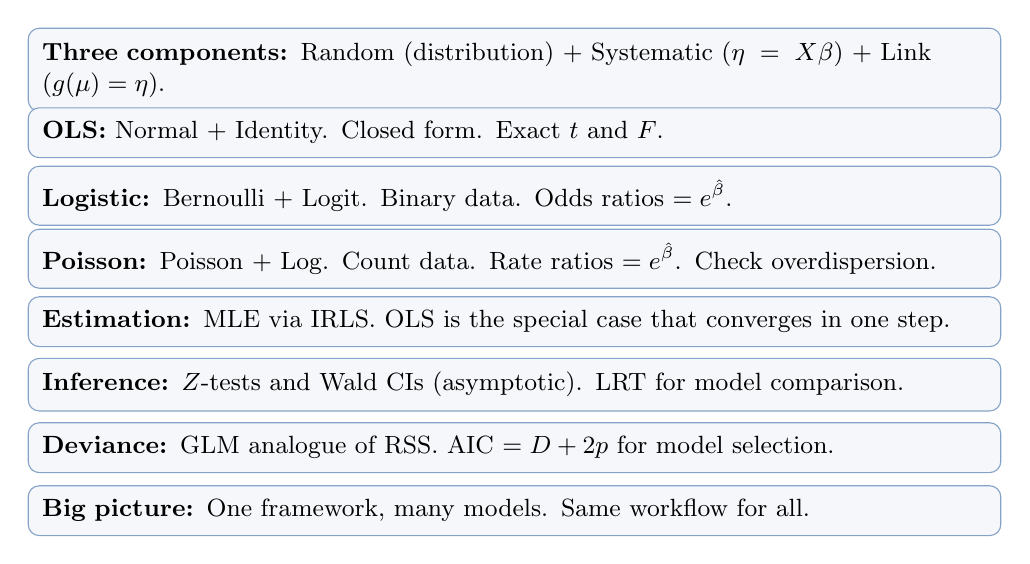
\begin{tikzpicture}[
  sbox/.style={draw=popblue!60, fill=popblue!5, rounded corners=4pt, text width=12cm, minimum height=0.5cm, align=left, inner sep=5pt, font=\small}
]
  \node[sbox] at (0, 3.2) {\textbf{Three components:} Random (distribution) + Systematic ($\eta = X\beta$) + Link ($g(\mu) = \eta$).};
  \node[sbox] at (0, 2.4) {\textbf{OLS:} Normal + Identity. Closed form. Exact $t$ and $F$.};
  \node[sbox] at (0, 1.6) {\textbf{Logistic:} Bernoulli + Logit. Binary data. Odds ratios $= e^{\hat\beta}$.};
  \node[sbox] at (0, 0.8) {\textbf{Poisson:} Poisson + Log. Count data. Rate ratios $= e^{\hat\beta}$. Check overdispersion.};
  \node[sbox] at (0, 0.0) {\textbf{Estimation:} MLE via IRLS. OLS is the special case that converges in one step.};
  \node[sbox] at (0, -0.8) {\textbf{Inference:} $Z$-tests and Wald CIs (asymptotic). LRT for model comparison.};
  \node[sbox] at (0, -1.6) {\textbf{Deviance:} GLM analogue of RSS. AIC $= D + 2p$ for model selection.};
  \node[sbox] at (0, -2.4) {\textbf{Big picture:} One framework, many models. Same workflow for all.};
\end{tikzpicture}
\end{center}
\end{frame}

% ============================================================
\section{Practical}

\begin{frame}
\frametitle{Practical: GLMs in Python}
\begin{center}
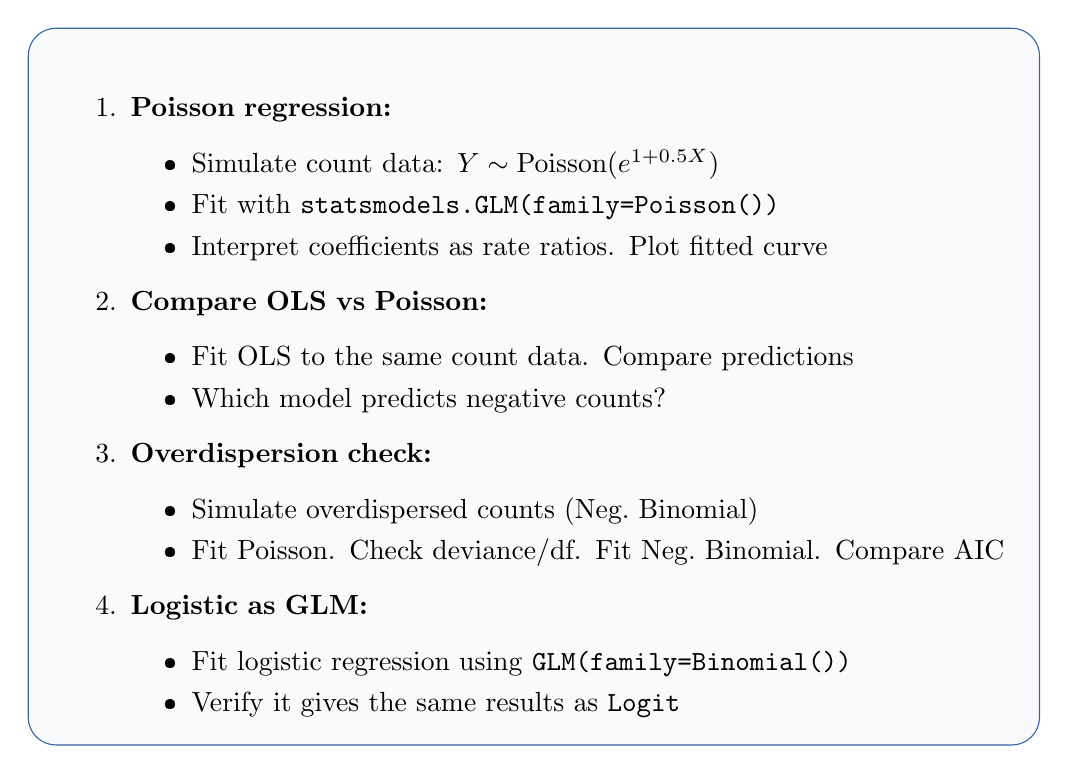
\begin{tikzpicture}
  \node[draw=popblue, fill=popblue!3, rounded corners=10pt, text width=12cm, align=left, inner sep=12pt] {
    \begin{enumerate}\setlength{\itemsep}{4pt}
      \item \textbf{Poisson regression:}
        \begin{itemize}\setlength{\itemsep}{1pt}
          \item Simulate count data: $Y \sim \text{Poisson}(e^{1 + 0.5 X})$
          \item Fit with \texttt{statsmodels.GLM(family=Poisson())}
          \item Interpret coefficients as rate ratios. Plot fitted curve
        \end{itemize}
      \item \textbf{Compare OLS vs Poisson:}
        \begin{itemize}\setlength{\itemsep}{1pt}
          \item Fit OLS to the same count data. Compare predictions
          \item Which model predicts negative counts?
        \end{itemize}
      \item \textbf{Overdispersion check:}
        \begin{itemize}\setlength{\itemsep}{1pt}
          \item Simulate overdispersed counts (Neg.\ Binomial)
          \item Fit Poisson. Check deviance/df. Fit Neg.\ Binomial. Compare AIC
        \end{itemize}
      \item \textbf{Logistic as GLM:}
        \begin{itemize}\setlength{\itemsep}{1pt}
          \item Fit logistic regression using \texttt{GLM(family=Binomial())}
          \item Verify it gives the same results as \texttt{Logit}
        \end{itemize}
    \end{enumerate}
  };
\end{tikzpicture}
\end{center}
\end{frame}

\begin{frame}
\frametitle{Homework}
\begin{enumerate}\setlength{\itemsep}{3pt}
  \item A hospital records daily ER visits ($Y$) with day of week and temperature.
    (a) Why is Poisson regression more appropriate than OLS?
    (b) Fit a Poisson GLM. Interpret coefficients as rate ratios.
    (c) Check for overdispersion. If present, refit with Neg.\ Binomial. Compare AIC.

  \item Show that for Normal($\mu$, $\sigma^2$) with known $\sigma^2$:
    (a) The canonical link is the identity.
    (b) The MLE is $\hat\mu = \bar{Y}$ (= OLS intercept-only).
    (c) The deviance equals RSS.

  \item A study models insurance claim amounts (positive, right-skewed).
    (a) Which GLM family and link would you use? Why?
    (b) Fit with \texttt{GLM(family=Gamma(link=Log()))}. Compare predictions with OLS.

  \item \textbf{Unifying exercise:} Take one dataset and fit OLS, logistic (binarize $Y$), and Poisson (round $Y$). Compare the \texttt{.summary()} tables.
\end{enumerate}
\end{frame}

\begin{frame}
\frametitle{Recommended Resources}

\footnotesize
\begin{center}
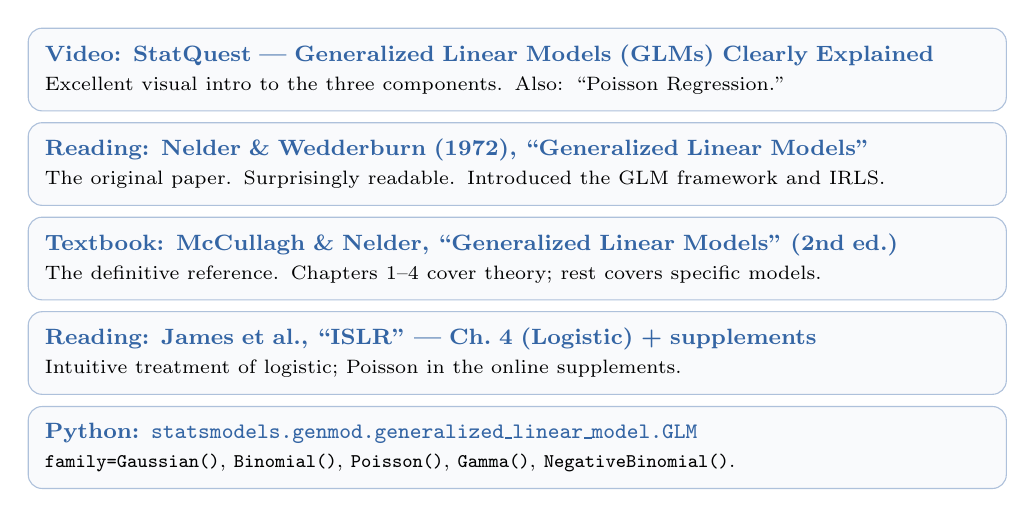
\begin{tikzpicture}[
  rbox/.style={draw=popblue!40, fill=popblue!3, rounded corners=5pt, text width=12cm, align=left, inner sep=6pt, font=\footnotesize}
]
  \node[rbox] at (0, 2.4) {
    \textbf{\textcolor{popblue}{Video: StatQuest --- Generalized Linear Models (GLMs) Clearly Explained}}\\[1pt]
    \scriptsize Excellent visual intro to the three components. Also: ``Poisson Regression.''
  };
  \node[rbox] at (0, 1.2) {
    \textbf{\textcolor{popblue}{Reading: Nelder \& Wedderburn (1972), ``Generalized Linear Models''}}\\[1pt]
    \scriptsize The original paper. Surprisingly readable. Introduced the GLM framework and IRLS.
  };
  \node[rbox] at (0, 0.0) {
    \textbf{\textcolor{popblue}{Textbook: McCullagh \& Nelder, ``Generalized Linear Models'' (2nd ed.)}}\\[1pt]
    \scriptsize The definitive reference. Chapters 1--4 cover theory; rest covers specific models.
  };
  \node[rbox] at (0, -1.2) {
    \textbf{\textcolor{popblue}{Reading: James et al., ``ISLR'' --- Ch.\ 4 (Logistic) + supplements}}\\[1pt]
    \scriptsize Intuitive treatment of logistic; Poisson in the online supplements.
  };
  \node[rbox] at (0, -2.4) {
    \textbf{\textcolor{popblue}{Python: \texttt{statsmodels.genmod.generalized\_linear\_model.GLM}}}\\[1pt]
    \scriptsize \texttt{family=Gaussian()}, \texttt{Binomial()}, \texttt{Poisson()}, \texttt{Gamma()}, \texttt{NegativeBinomial()}.
  };
\end{tikzpicture}
\end{center}
\end{frame}

\begin{frame}
\begin{center}
  {\Huge\bfseries\textcolor{popblue}{Questions?}}

  \vspace{1cm}

  {\large Next: Lecture~14 --- Causal inference}
\end{center}
\end{frame}

\end{document}
